%!TEX root = ../masters.tex

\chapter{Introdução}
\label{cha:introduction}


\begin{figure}
	\centering
	\caption{Processo de Extração de Metadados}
	\label{fig:introduction}
	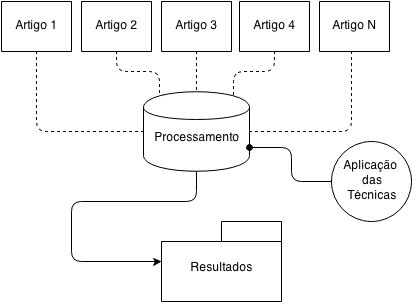
\includegraphics[width=0.7\linewidth]{./assets/images/introduction}
\end{figure}

\section{Contexto}
\label{sec:context}

A eficácia no armazenamento de artigos requer análise automatizada de seus conteúdos de maneira a extrair as partes mais importantes, como título, autores e referências. Assim eles poder ser catalogados de maneira organizada e estruturada, que facilita a busca posterior. 
Estes dados retirados dos documentos analisados são referenciados neste projeto pelo nome de ``metadados'', e são detalhados mais a frente de maneira aprofundada.

A pesquisa aqui realizada situa-se no campo da extração de metadados principalmente via \textit{machine learning}. Este trabalho aborda as principais ferramentas encontradas atualmente. Diversas ferramentas e técnicas para extração de metadados em artigos podem ser encontradas na Internet. Algumas são propriedade de universidades ou instituições privadas, o que dificulta a análise. Algumas ferramentas não permitem que testes automatizados sejam feitos, visto que não permitem acesso ao código fonte ou não podem ser utilizadas via linha de comando, dificultando a análise dos resultados.

De modo geral, as ferramentas de extração são focadas em \textit{layouts} (disposição visual) pré-definidos, geralmente seguindo modelos de conferências e/ou congressos internacionais, que possuem um padrão visual já estabelecido, como é o caso do IEEE (\textit{Institute of Electrical and Electronics Engineers}), por exemplo, que serve de referência para diversos outros eventos da área da computação, tomando seu \textit{layout}, a princípio, como base.

Porém, existem diversos outros eventos que possuem \textit{layouts} de artigos fora de padrão que necessitam de adaptações por parte das ferramentas para serem analisados e catalogados de maneira automática. 

Algumas ferramentas são aparentemente muito eficazes para um certo grupo de artigos, já seguindo um padrão visual pré-determinado. Porém, para alguns \textit{layouts} pouco comuns, de áreas do conhecimento diversas, espera-se que estas ferramentas não sejam tão eficazes, variando de acordo com a tecnologia utilizada e, principalmente, de acordo com o princípio teórico utilizado pelos seus autores, que será mais aprofundado nos próximos capítulos.

Como definido por \cite{foundations-machine-learning}, \textit{machine learning} permite uma forma de aprendizado com base em experiências passadas, através da utilização de dados coletados, que são analisados posteriormente seguindo padrões definidos.

Este tema é muito amplo e sua aplicabilidade é diversificada, permitindo a utilização de suas técnicas e teorias em diversas atividades, como classificação de textos e documentos, processamento de linguagem natural, reconhecimento de fala, detecção de fraudes, diagnósticos médicos e sistemas de recomendações, além de mecanismos de buscas e extração de informação, ponto principal de discussão deste trabalho.

O objetivo da pesquisa é identificar quais são as melhores ferramentas de extração de metadados em artigos científicos e suas melhores aplicações, com base em um conjunto de documentos pré-selecionados para testes, dos mais diversos padrões e de diversas áreas do conhecimento.

Com efeito, esta identificação permite que resultados sejam comparados e confrontados, para decidir qual ferramenta é melhor utilizada para cada padrão visual, abrangendo um conjunto cada vez maior de dados e tendo resultados cada vez mais precisos.

Com base na diferenciação dos \textit{layouts} de artigos científicos, este trabalho visa identificar também pontos em que as ferramentas de extração de metadados necessitam de adaptações por parte de seus usuários e desenvolvedores, permitindo, garantindo assim, uma cobertura mais abrangente dos artigos científicos. Além disso, com base nos resultados coletados, pode-se identificar qual ferramenta é melhor aplicada para cada tipo distinto de metadado.

Acredita-se que os padrões de extração existentes hoje são, de maneira geral, insuficientes para suprir todos os \emph{layouts} de artigos existentes, limitando a apenas uma pequena parcela destes, dentro de um padrão visual específico.

As formas de extração de metadados em artigos científicos são geralmente baseadas em \textit{layouts}, ou seja, em pequenos pedaços de documentos onde certos dados devem estar presentes. Porém, em virtude da diversidade de materiais produzidos, dos mais diversos padrões visuais e áreas do conhecimento, este \textit{layout} padrão não se mostra eficiente na abrangência total das necessidades da comunidade científica como um todo. 

Sobre este aspecto, espera-se que certos artigos científicos não tenham seus metadados extraídos de maneira precisa por todas as ferramentas analisadas, uma vez que adaptações no código seriam necessárias a fim de permitir que outros padrões visuais de artigos fossem também reconhecidos, aplicando então um dos fundamentos do \textit{machine learning}, o aprendizado por repetição. 

Por fim, espera-se que, com esta análise aprofundada das ferramentas selecionadas, as mais eficazes na extração de metadados sejam identificadas e analisadas, elevando então o ganho científico neste tema importante para o desenvolvimento tecnológico.

O documento é estruturado iniciando com uma breve introdução sobre o tema.
O segundo capítulo tem como base o referencial teórico feito através de um mapeamento de bases de dados e eventos científicos relevantes para a área. Neste capítulo são apresentados alguns conceitos básicos, além das técnicas mais utilizadas e as ferramentas mais comuns encontradas atualmente.

O terceiro capítulo apresenta a metodologia usada no trabalho. Cita as ferramentas que serão testadas e principalmente como serão feitos os testes. 

Posteriormente, no capítulo quarto faz-se a análise e apresentação dos resultados, explicando como os testes foram realizados, os ambientes de teste criados e os resultados coletados.

No quinto capítulo temos a discussão/conclusão, trabalhos futuros e considerações finais sobre o trabalho apresentado.


%\section{Limitações do Trabalho}
%
%Este trabalho limita-se aos artigos científicos difundidos na comunidade científica em formato PDF, excluindo aqueles em que seu conteúdo é disponibilizados através de imagens escaneadas de documentos físicos, o que impede, em um primeiro momento, de ter os textos analisados em sua forma original, sem necessidade de processamento extra a fim de obter todo o material textual contido em tais imagens. Além disso o trabalho pressupõe que a língua inglesa seja utilizada como padrão
%
%% Sobre os servidores com Windows
%
%Já na questão de testes de cada técnica de extração de metadados, as técnicas que serão selecionadas deverão ser de código livre/aberto, ou seja, ter seu uso liberado sem a necessidade de pagamento de licenças. Deste modo excluímos todas as técnicas que necessitam de \textit{softwares} proprietários para funcionar, por exigir licenças e fugirem das previsões de teste deste projeto. Assim, os projetos deverão necessariamente utilizar de linguagens de programação livres (ou de código aberto) e que rodem em sistemas operacionais derivados do Unix, como o Linux, por exemplo.


